%%%% hw3-reqdoc.team3.tex
%%%% Requirements Documentation for sQuire
%%%% Due on BBLearn before class on Tuesday 2/9/2016

\documentclass[11pt]{report}

\usepackage{graphicx}
%\graphicspath{ {images/} }

\marginparwidth 0.5in 
\oddsidemargin 0.25in 
\evensidemargin 0.25in 
\marginparsep 0.25in
\topmargin 0.0in 
\textwidth 6in \textheight 8.5in

\title{sQuire: A Collaborative Software Development Tool}
\author{jank6275, mora5651, boss2849, bolt1003, gall7417, brec9824, snev7821, mars2681}

\begin{document}

\maketitle

\tableofcontents

\chapter{Introduction}

\section{Program Premise}
    \begin{figure}[h!]
        \caption{Squire will be a web-based collaborative software development environment with a project development center. Squire will allow multiple users to edit files and communicate in real time. First, projects are stubbed out by a user and then other users can join and/or vote to support for their favorite projects. After a certain amount of support, planning, and documentation is reached for a project, the project becomes a fully fleged project and then community development can start. Think ``kickstarter for code'' where people pledge their help with the project and not just money.}
        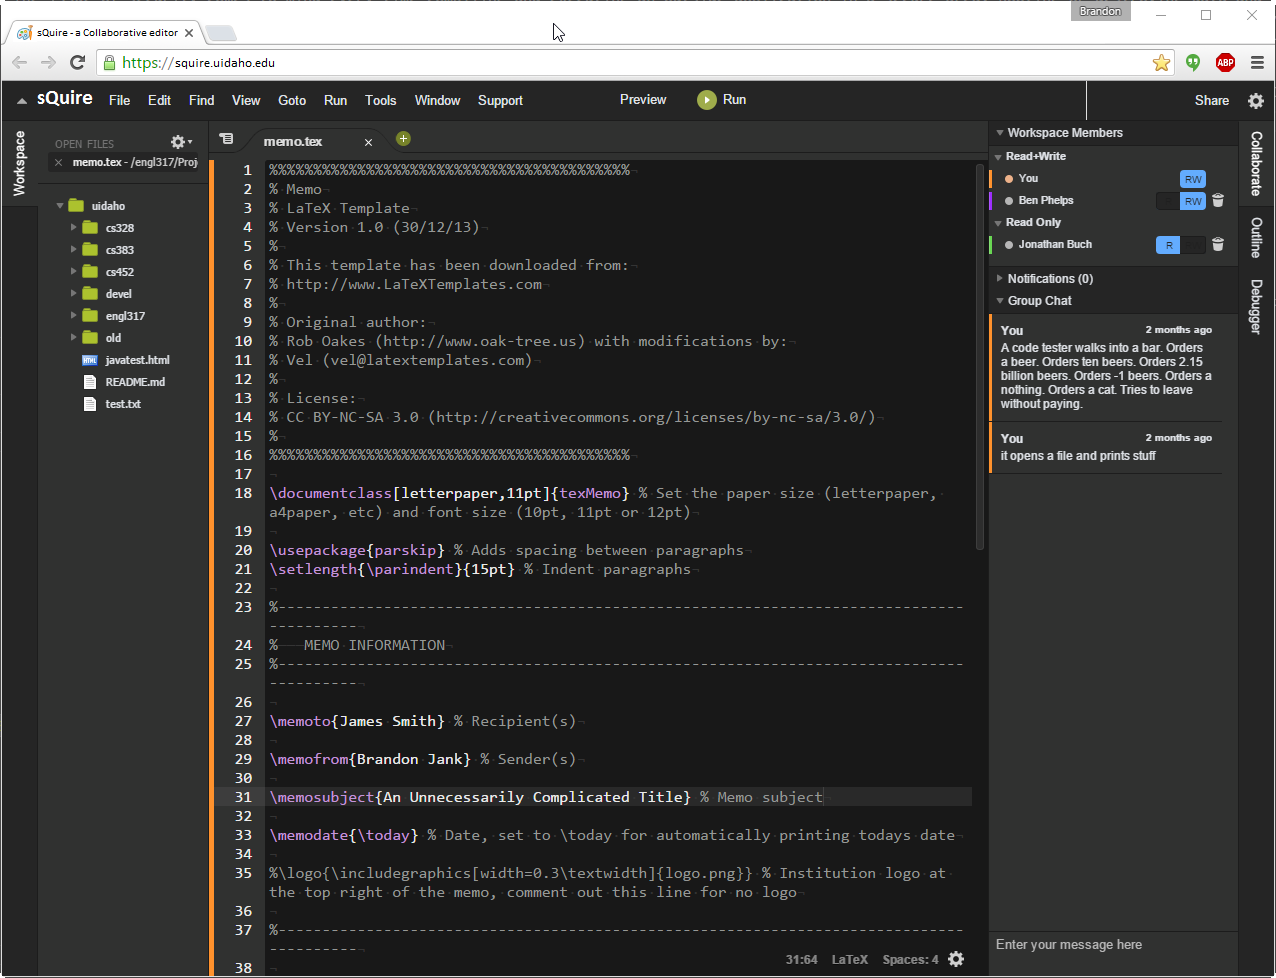
\includegraphics[width=\textwidth]{squire}
    \end{figure}

\section{Use Case Overview (jank6275)}
    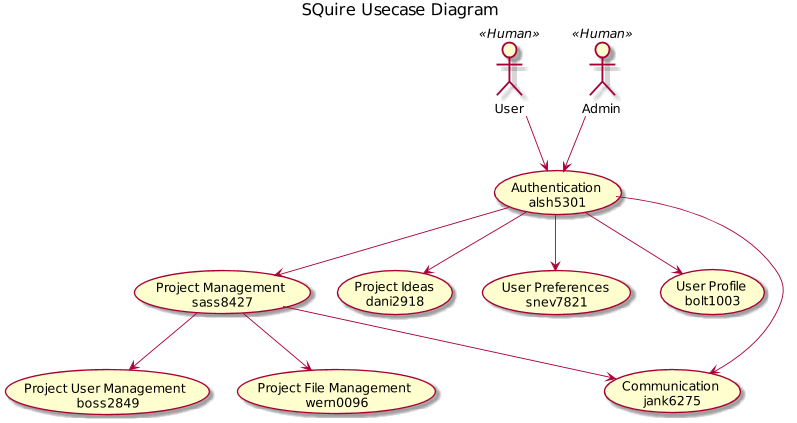
\includegraphics[width=\textwidth]{diagrams/overview-jank6275}
    A usecase diagram that shows all of sQuire\'s features.

\chapter{Requirements Documentation}

\section{Functional Requirements}
    Functional requirements will specify a behaviour or function, for example ``Display the name, total size, available space and format of a flash drive connected to the USB port'' Other examples are ``add customer'' and ``print invoice''. Some of the more typical functional requirements include:
    
    \subsection Authentication (mars2681)
        \begin{itemize}
            \item First, the user can input their email address and password in order to sign into their account. If they do not have an account, they can sign up by providing an email address and a password. A confirmation email will then be sent to their email address, which they can use to confirm and access their account. If the user forgets their password, they can click “forgot password” and input their email address. The system with confirm an email addresses associated with an account, and email the user a temporary password. 
        \end{itemize}
    \subsection Project Management (mora5651) 
        \begin{itemize}
            \item Admin controls features.  
            \item Public and private sharing of project.
            \item Controlled reading and writing permissions to users. 
            \item Password controls. 
            \item File management. 
        \end{itemize}
    \subsection Project Ideas (snev7821) 
        \begin{itemize}
            \item Forum to browse potential projects
            \item Up- and down-votes for project selection
            \item Different ways to sort projects (date, projected team size, votes)
            \item Ability to post a project
            \item Ability to delete a project (but only by project author)
            \item Convert potential project stub into active working project 
        \end{itemize}
    \subsection User Profile (brec9824) 
        \begin{itemize}
            \item Viewable profile by other users and by oneself
            \item Includes editable email, profile image, password, and personal bio.
            \item Setting for public, friends only, or private viewing of online status, email address, personal bio, project ownerships, project memberships, and friends list.
            \item Option for settings users prefered color and shape to be displayed in projects if available.
            \item Option to have account deleted.
        	\item Direct access to projects that are listed under project ownerships and project memberships.
        \end{itemize}
    \subsection Project File Editor (jank6275) 
        \begin{itemize}
            \item The editor will be multi-user, up to 32 users can share an IDE session.
            \item Text will be underlined in the user\'s color, if they edited/created that text.
            \item The line number will be highlighted in the users color, if they created the line.
            \item Each line edited by a user should be saved to create a edit history for each user in a document.
            \item Users will be able to edit the same document concurrently.
            \item Any user can save the document at any time.
            \item The current location of any user\'s cursor can be quickly jumped to by any user with the project open.
        \end{itemize}
    \subsection Communication (bolt1003) 
        \begin{itemize}
            \item Built-in, global text chat per project.
            \item Private communications between other users.
            \item A friends list with friend status icons and avatar.
            \item A global list of current memembers in the project.
            \item A list of current users working on the project.
            \item A dialog with the user\'s name and file history when hovering over their icon.
            \item Text chat will be built using standard protocols such as XMPP or IRC.
            \item Allows the use of third-party chat clients.
        \end{itemize}
    \subsection Security (gall7417) 
        \begin{itemize}
            \item Resource defense strategy that includes not subjecting any sQuire server to becoming unresponsive due to a runaway program, and not allowing any sQuire server to give up shell access via an executing program in sQuire.
            \item Require authentication to access all user files and user information.
            \item Ensure confidentiality of all user information.
            \item Use password hashing on a trusted system to ensure password privacy.
            \item Hide password entry on user interface.
            \item Allow password change and reset in case of compromise.
            \item Mitigate security threats by testing against common abuse cases and vulnerabilities.
            \item Validate user integrity before any processing is performed.
            \item Ensure proper character sets for all input given.
            \item All validation failures must result in rejection.
            \item Implement a force halt procedure for runaway programs.
            \item Establish system inactivity timeout after arbitrary amount of time.
            \item Enforce authorization controls on all system requests.
            \item Restrict access to resources and files outside of the users given resources.
            \item Deny access to security protocols and configurations.
        \end{itemize}
    \subsection Compiler (boss2849) 
        \begin{itemize}
            \item Capable of supporting editing, compilation, and execution of Java programs. Programs to be composed as projects and support multiple source code files across multiple directories within a shared top-level directory.
            \item Design as a 'plugin' to the system - initial will be a Java compiler, but allow new compiler plugins to be written for other languages.
            \item Compile code for execution within IDE.
            \item Compile code and package to a JAR.
            \item Compile file, file and dependents, project sub-modules, or entire project.
            \item Smart compilation - recompile only what has been changed. 
            \item Allow temporary code freeze before compilation.
            \item Cache snapshots of code on compilation. 
        \end{itemize}
    
\section{Non-Functional Requirements}
    Non-functional requirements cover all the remaining requirements which are not covered by the functional requirements. They specify criteria that judge the operation of a system, rather than specific behaviours, for example: ``Modified data in a database should be updated for all users accessing it within 2 seconds.'' Some typical non-functional requirements are:
    
    \begin{itemize}
        % Performance – for example Response Time, Throughput, Utilization, Static Volumetric (jank6275)
            \item Squire should perform good, and stuff. (jank6275)
        % Scalability (boss2849)
            \item Scalability is important to keep in mind during development. The system should be designed in such a way that will easily and reliably scale to accommodate a growing user base. One method of dealing with scalability would be allowing the core system to reactively spawn new slaves to aid in computational needs, such as compilation (as that will be more resource intensive the user base grows). (boss2849)
        % Capacity  
            \item Limited space for projects that haven\'t been initiated (enough for documentation, images, etc.) (boss2849)
            \item Reactively increasing capacity for projects proportional to the absolute needs of the projects. (no fluff) (boss2849)
            \item Encourage developers to store large files elsewhere, e.g. GitHub LFS, AWS, etc. (boss2849)
        % Availability (brec9824) 
            \item Since sQuire is web based, downtime for the servers most be kept to a minimum and be no more then once or twice a week for a few hours. This downtime will allow for database uprgrades and backups. (brec9824)
        % Reliability (bolt1003) 
            \item sQuire will be a web application and will leverage the strengths of web technologies to make it reliable.       sQuire will use a webhost such as, Amazon Web services. The webhost\'s infrastructure provides, redunancy for hardware, power and internet service. (bolt1003)
        % Recoverability (mora5651) 
            \item SQuire will have the ability for the user to save on sQuire\'s database for recoverability isurance. It will also incorporate autosave feature. (mora5651)
        % Maintainability (mora5651) 
            \item Since sQuire is a web based application running on a webhost. There are 
            many maintenance tools that can be used to track performance. Maintainability of sQuire will also include regular backup schedules, speed test, and security monotoring. (mora5651)
        % Serviceability (bolt1003) 
            \item Running sQuire as a web application allows it to quickly and easily rollback to a previous version or rollforward to a new version. This allows for rapid bug fixing. Infrastructure is redunane so equipment can be taken offline for repair without interupting the users. (bolt1003)
        % Security (jank6275)
            \item Docker, dokku-alt, docker, dokku, docker. (jank6275)
        % Regulatory (mars2681) 
            \item Before the user can create an account, they have to agree with several laws. They must comply with the DMCA, and agree that any projects they create that are subjected to copyright violation isn’t associated with sQuire. They must also confirm they are over 18 years of age, complying with COPPA law. (mars2681)
        % Manageability (brec9824) 
            \item Will include monitoring of subsystems to collect and report performance data. (brec9824)
            \item Subsystem monititory must be highly efficient and take up less than 10\% of resources to keep noticeability to a minimum. (brec9824)
            \item Subsystems must be modular to allow for efficient monitoring, implementation of subsystems, and the addition of new subsystems. (brec9824)
        % Environmental (gall7417) 
            \item sQuire will run as a browser application in google chrome. (gall7417)
            \item sQire will run on virtually all modern processors. (gall7417)
        % Data Integrity (gall7417) 
            \item sQuire will use tcp to for reliable data communications. (gall7417)
            \item sQuire will use error checking upon large changes to ensure no drastic data corruption occurs. (gall7417)
            \item sQuire will use a history/autosave feature in case of data loss. (gall7417)
        % Usability (snev7821) 
            \item Provides code compilation and file system for users with limited resources. (snev7821)
            \item Easy to learn system, helpful syntax highlighting. (snev7821)
            \item More satisfying than competitors products, because of social/kickstarter aspect. (snev7821)
        % Interoperability (snev7821) 
            \item Provides github integration. (snev7821)
            \item Runs on any of the main browsers (chrome, firefox, IE, safari). (snev7821)
            \item Due to web based design, works on lower end machines. (snev7821)
    \end{itemize}

\section{Unused Requirements}
    \begin{itemize}
        \item Since multiple people might edit a given line over its history, support for past history or anyhow multiple persons in this indication is strongly recommended.
        \item Teams should decide if voice or video is essential. Voice, if supported, might be restricted as to number of listeners and/or number of simultaneous transmitters. Video, if supported, might be restricted as to number of viewers and/or number of simultaneous. - NO, we have skype for a reason.
    \end{itemize}
    
\end{document}